\chapter{Introduction}
\label{ch:intro}

\textit{The limits of my language means the limits of my world.}  \\
\noindent\textbf{-Ludwig Wittgenstein}

\vspace{1cm}
\begin{marginfigure}%
  \includegraphics[width=\linewidth]{clock.jpg}
  \caption{Exploded clock assembly}
  \label{fig:marginfig}
\end{marginfigure}



\newthought{Physics is embodied} through the process of measurement.  Within physics any meaningful statement relates to some observable quantity.  The process of observation requires measurement using physical instrumentation.  In this way, physics is not only about the world but made of the world.
\begin{marginfigure}%
 \Large $$ E=hf$$
  \caption{Mathematical equation relating the energy and oscillatory frequency of a radiant particle.}
  \label{fig:marginfig}
\end{marginfigure}

\newthought{Physics is symbolic} in the application of mathematics to the working world.   Observable quantities are represented by algebraic variables and .  Once quantities are abstracted as mathematical variables, physics becomes a language game.

\newthought{Physics is visual} in both the measurement and the representation.
\begin{marginfigure}%
  \includegraphics[width=\linewidth]{bubble.jpg}
  \caption{Bubble chamber image of a neutrino particle interaction event from the Fermi National Accelerator Laboratory.}
  \label{fig:marginfig}
\end{marginfigure}
\newthought{Physics is social}.   In the end mathematics and physical observation are human activities.  As is Soylent Green, physics too is made of people.  People!  This does not mean we can not gain insights beyond ourselves.  Hopefully it means physicists will have jobs.
\begin{marginfigure}%
  \includegraphics[width=\linewidth]{feyn.jpg}
  \caption{Feynman diagram representing photon mediated electron-electron scattering.}
  \label{fig:marginfig}
\end{marginfigure}

\section{Quantities}
\newthought{A physical quantity is} a physical property of a phenomenon, body, or substance, that can be quantified by measurement.  We can represent a physical quantity using an algebraic variable.  A physical quantity requires a value and unit of measure.
$$t = \overbrace{153}^{\textit{Value}} \ \ \overbrace{\text{seconds}}^{\textit{Unit}}$$
Consider the physical quantity, time.  In the above equation we use $t$ as the algebraic variable, seconds as the unit of measure and 153 as the value or magnitude of that unit.
\marginnote{\textit{So Simon Peter climbed back into the boat and dragged the net ashore. It was full of large fish, 153, but even with so many the net was not torn.}
\textbf{- John 21:11}}
\vspace{1cm}
$$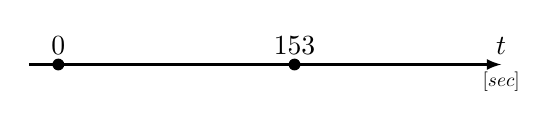
\begin{tikzpicture}[scale=1.5]
   \draw[->,thick,-latex] (0,0) -- (4,0) node [anchor=north ,scale=0.7] {$[\text{sec}]$}node [anchor=south ,scale=1] {$t $}; 
    %  \draw[->,-latex] (1.25,0.15) -- (2.75,0.15)  node [black,midway,above=0pt,yshift=2pt] { $\Delta_1 x_i$}; 
   \fill[black] (0.25,0) circle (0.5mm) node [anchor=south ,scale=1] {$0$};
    \fill[black] (2.25,0) circle (0.5mm) node [anchor=south ,scale=1] {$153$};
   
   \end{tikzpicture}
   $$
   \marginnote[-10pt]{The \textbf{accuracy} of a measurement system is the degree of closeness of measurements of a quantity to that quantity's true value.  The \textbf{precision} of a measurement system, related to reproducibility and repeatability, is the degree to which repeated measurements under unchanged conditions show the same results.}
The same information in the above equation may be encoded graphically using an appropriately labeled number line.  Here the quantity's magnitude may be represented a length measured by a point and the origin.

\subsection{Scientific Notation}
Scientific notation is a way of writing numbers that are too big or too small to be conveniently written in decimal form.  In scientific notation the numerical value 153 would be written as $1.53\times10^2$.

$$153= \overbrace{1.53}^{\text{significant figures}} \ \times\ \overbrace{10^2}^{\text{order of magnitude}}$$

In this format only one non-zero digit is to the left of the decimal place and to the right of the decimal place go the remaining significant figures.  The order of magnitude is the exponent power of ten.  In this example there are three significant figures and an order of magnitude of two.  Scientific notation enables simpler order-of-magnitude comparisons.


\begin{margintable}[20pt]\index{typefaces!sizes}
  \footnotesize%
  \begin{center}
    \begin{tabular}{lc}
      \toprule
     Length & Meters \\
      \midrule
     Observable Universe     & $10^{26}$  \\
    Milky Way      & $10^{21}$  \\
    Solar System     & $10^{13}$  \\
    Earth to Sun    & $10^{11}$  \\
    Earth     & $10^{7}$  \\
    Football Field      & $10^{2}$  \\
    Human      & $10^{0}$  \\
    Cell     & $10^{-5}$  \\
    Hydrogen Atom      & $10^{-10}$  \\
    Proton      & $10^{-15}$  \\
      \bottomrule
    \end{tabular}
  \end{center}
  \caption{A list of length scales.}
  \label{tab:font-sizes}
\end{margintable}

\begin{margintable}[20pt]\index{typefaces!sizes}
  \footnotesize%
  \begin{center}
    \begin{tabular}{lc}
      \toprule
     Time & Seconds\\
      \midrule
    Age Universe     & $10^{17}$  \\
    Age Earth      & $10^{17}$  \\
    Life on Earth      & $10^{17}$  \\
     Year    & $10^{7}$  \\
    Month    & $10^{6}$  \\
    Day     & $10^{5}$  \\
    Sunlight to Earth      & $10^{2}$  \\
    Heartbeat      & $10^{0}$  \\
    Audible Latency    & $10^{-2}$  \\
    Pion Lifetime      & $10^{-8}$  \\
      \bottomrule
    \end{tabular}
  \end{center}
  \caption{A list of time scales.}
  \label{tab:font-sizes}
\end{margintable}

\subsection{Approximation}
\newthought{Making order of magnitude approximations} involves using these $10^n$ representations.  Consider for example a deep breathing yogi.  How many breaths do they take per day?  The time scale for a breath is on the order of 10  or $(10^1)$ seconds while a day is on the order of $10^5$ seconds.  Therefore the number of breaths per day would be on the order of $10^4$, or ten thousand breaths.

$$\frac{10^5}{10^1}=10^{5-1}=10^4$$

Said another way, the time for the rotation of the earth is four orders of magnitude greater than the cycle of the breath.



\newpage
\subsection{Units and Dimensions}
\marginnote[20pt]{The \textit{International System of Units} (\textbf{SI}) is the modern form of the metric system and is the world's most widely used system of measurement, used in both commerce and science. It comprises a coherent system of units of measurement built on seven base units. It defines twenty-two named units, and includes many more unnamed coherent derived units. The system also establishes a set of twenty prefixes to the unit names and unit symbols that may be used when specifying multiples and fractions of the units.}


\begin{margintable}[20pt]\index{typefaces!sizes}
  \footnotesize%
  \begin{center}
    \begin{tabular}{lccl}
      \toprule
     Prefix & Symbol & Value \\
      \midrule
     yotta  & Y      & $10^{24}$  \\
    zetta  & Z      & $10^{21}$  \\
    exa    & E      & $10^{18}$  \\
    peta   & P      & $10^{15}$  \\
    tera   & T      & $10^{12}$  \\
    giga   & G      & $10^{9}$   \\
    mega   & M      & $10^{6}$   \\
    kilo   & k      & $10^{3}$   \\
    hecto  & h      & $10^{2}$   \\
    deca   & da     & $10^{1}$   \\ 
    deci   & d      & $10^{-1}$  \\
    centi  & c      & $10^{-2}$  \\
    milli  & m      & $10^{-3}$  \\
    micro  & $\mu\ $ & $10^{-6}$  \\
    nano   & n      & $10^{-9}$  \\
    pico   & p      & $10^{-12}$ \\
    femto  & f      & $10^{-15}$ \\
    atto   & a      & $10^{-18}$ \\
    zepto  & z      & $10^{-21}$ \\
    yocto  & y      & $10^{-24}$ \\
      \bottomrule
    \end{tabular}
  \end{center}
  \caption{A list of metric prefixes.}
  \label{tab:font-sizes}
\end{margintable}
\begin{description}
\item[meter] The meter is the length of the path travelled by light in vacuum during a tim interval of $1/299,792,458$ of a second.
\item[kilogram] The kilogram is the unit of mass; it is equal to the mass of the international prototype of the kilogram.
This international prototype is made of platinum-iridium and is kept at the International Bureau of Weights and Measures in France.
\item[second] The second is the duration of $9,192,631,770$ periods of the radiation corresponding
to the transition between the two hyper fine levels of the ground state of the cesium-133 atom.
\item[ampere] The ampere is that constant current which, if maintained in two straight parallel
conductors of infinite length, of negligible circular cross-section, and placed
one meter apart in vacuum, would produce between these conductors a force
equal to $2\times10^{-7}$ newton per meter of length.
\item[kelvin] The kelvin, unit of thermodynamic temperature, is the fraction 1/273.16 of the
thermodynamic temperature of the triple point of water.
\item[mole] The mole is the amount of substance of a system which contains as many
elementary entities as there are atoms in $0.012$ kilogram of carbon 12.  When the mole is used, the elementary entities must be specified and may be atoms, molecules, ions, electrons, other particles or specified groups of such particle.
In this definition, it is understood that the carbon 12 atoms are unbound, at rest and in their ground state.
\item[candela] The candela is the luminous intensity, in a given direction, of a source that emits
monochromatic radiation of a frequency $540\times10^{12}$ Hertz and has a radiant intensity in that direction of $1/683$ watt per steradian.
\end{description}



\begin{table}[htbp]
\begin{center}
\footnotesize
\begin{tabular}{lllll}
\toprule
Quantity & SI Unit & SI Symbol & Variable & Dimension  \\
\midrule
Fundamental & &  \\
\quad  distance & meter     & m           & $l$    &   $\mathbf{L}$          \\
\quad   mass &  kilogram  & kg          &      $m$       & $\mathbf{M}$        \\
\quad   time            & second    & s           &    $t$     &   $\mathbf{T}$      \\
\quad  electrical current &ampere &   A           &  $I$ &   $\mathbf{I}$    \\
\quad  temperature & kelvin    & K           &  $T$ &  $ \mathbf{\Theta} $ \\
\quad   number particles &   mole      & mol         &   $n$   &  $ \mathbf{N}$     \\
\quad  luminous intensity   & candela   & cd          &    $J$& $\mathbf{J}$      \\ \addlinespace
Derived & &  \\
\quad angle      &radian    & rad &$\theta$        &     $\mathbf{1}$           \\
\quad     frequency    &hertz     & Hz = $\nicefrac{1}{\text{s}}$         &      $f$ & $\mathbf{T}^{-1}$ \\
\quad    force & newton    & N   = $\nicefrac{\text{kg}\cdot \text{m}}{\text{s}^2}$        & $F$ & $\mathbf{M}\mathbf{L}\mathbf{T}^{-2}$           \\
\quad  pressure &  pascal    & Pa  = $\nicefrac{\text{N}}{\text{m}^2}$        &     $P$   & $\mathbf{M}\mathbf{L}^{-1}\mathbf{T}^{-2}$  \\
\quad   energy        &  joule     & J   = $\text{N} \cdot \text{m}$        &     $E$ & $\mathbf{M}\mathbf{L}^{2}\mathbf{T}^{-2}$\\
\quad    power       & watt      & W  = $\nicefrac{\text{J}}{\text{s}}$         &     $P$ & $\mathbf{M}\mathbf{L}^{2}\mathbf{T}^{-3}$  \\
\quad    electric charge  & coulomb   & C = $\text{A} \cdot \text{s}$           &   $q$& $\mathbf{I}\mathbf{T}$\\
\quad    electric potential & volt      & V = $\nicefrac{\text{J}}{\text{C}}$           & $V$& $\mathbf{M}\mathbf{L}^{2}\mathbf{T}^{-3}\mathbf{I}^{-1}$\\
 \quad  capacitance     & farad     & F = $\nicefrac{\text{C}}{\text{V}}$          &     $C$  & $\mathbf{M}^{-1}\mathbf{L}^{-2}\mathbf{T}^{4}\mathbf{I}^{2}$\\
 \quad   resistance   &ohm       & $\Omega$ = $\nicefrac{\text{V}}{\text{A}}$   &     $R$  & $\mathbf{M}\mathbf{L}^{2}\mathbf{T}^{-3}\mathbf{I}^{-2}$\\
 \quad   magnetic field    & tesla     & T  = $\nicefrac{\text{V}\cdot \text{s}}{\text{m}^2}$         & $B$   & $\mathbf{M}\mathbf{T}^{-2}\mathbf{I}^{-1}$ \\
\quad    inductance    & henry     & H = $\nicefrac{\text{V}\cdot \text{s}}{\text{A}}$         &   $L$ & $\mathbf{M}\mathbf{L}^{2}\mathbf{T}^{-2}\mathbf{I}^{-2}$ \\
 \quad  radioactivity  & becquerel & Bq = $\nicefrac{1}{\text{s}}$           & $A$  & $\mathbf{T}^{-1}$   \\ 
\bottomrule
\end{tabular}
\end{center}
  \caption{A list of physical quantities with SI units and dimensions.}
  \label{tab:font-sizes}
\end{table}

\newpage
\newthought{Any physical quantity} $Q$ is proportional to a product of fundamental quantities.  The critical exponents always being integer values.
 $$Q=Cl^\alpha m^\beta t^\gamma I^\delta T^\epsilon n^\xi J^\eta$$
\marginnote[-150pt]{The concept of physical dimension was introduced by Joseph Fourier in 1822.  Physical quantities that are commensurable have the same dimension; if they have different dimensions, they are incommensurable. For example, it is meaningless to ask whether a kilogram is less, the same, or more than an hour.  Any physically meaningful equation will have the same dimensions on the left and right sides, a property known as "dimensional homogeneity".}
The dimension of the quantity, $\text{dim }Q$, is a product of the dimensions of the constituent quantity factors.  
 $$\text{dim }Q=\mathbf{L}^\alpha \mathbf{M}^\beta \mathbf{T}^\gamma \mathbf{I}^\delta \mathbf{\Theta}^\epsilon \mathbf{N}^\xi \mathbf{J}^\eta$$
 \marginnote[-30pt]{Here $\alpha$, $\beta$, $\gamma$, $\delta$, $\epsilon$, $\xi$, $\eta$ are all positive or negative integers}
 This constitutes what is called and Abelian group.
 
\paragraph{Algebra and Similitude}
A sum or difference of two commensurate quantities (having the same dimensions) is a physically meaningful expression.
$$402\   \text{meter} -137\   \text{meter}=(402-137) \text{meter}=265\  \text{meter}$$
A product or quotient of any quantities can be a physically meaningful expression.
$$\frac{265\ \text{meter}}{153\ \text{second}}=\frac{265}{153}\ \frac{\text{meter}}{\text{second}}=1.73\  \nicefrac{\text{m}}{\text{s}}%\approx \sqrt{3}\ \nicefrac{\text{m}}{\text{s}}
$$

\paragraph{Unit Conversion}
\marginnote[-120pt]{The conversion of a quarter mile into meters.
\begin{align*} 
0.25\  \text{mi } \underbrace{\left(\frac{1609 \text{ m} }{ 1 \text{ mi}}\right)}_{\large{1}}&=\frac{0.25\cdot 1609}{1} \  \cancel{\text{mi}} \frac{\text{m} }{\cancel{\text{mi}}} \\
0.25\  \text{mi } &=402 \text{ m}
\end{align*}
}
\begin{margintable}[-30pt]\index{typefaces!sizes}
  \footnotesize%
  \begin{center}
    \begin{tabular}{lccl}
      \toprule
     English $\Longleftrightarrow$ Metric                                             \\
      \midrule
    $1 \text{ mile} = 5280 \text{ feet} = 1609 \text{ meters}$  \\
    $1 \text{gallon} = 3.785 \text{ liters} = 4.000 \text{ quarts}$                \\
    $1 \text{ cm}^3= 1 \text{ milliliter}$                                         \\
    $1 \text{ hp} = 746 \text{ Watts}$                                             \\
    $1 \text{ lb} = 4.45 \text{ Newtons}$                                          \\ 
      \bottomrule
    \end{tabular}
  \end{center}
  \caption{English and Metric equivalences}
  \label{tab:font-sizes}
\end{margintable}



The dimensions of a conversion factor are unity.  Any physically meaningful equality can be turned into one of two conversion factors.
$$1 \text{ mile} = 1609 \text{ meters} \ \ \ \ \ \Longleftrightarrow \ \ \ \ \ \frac{1609 \text{ meters} }{ 1 \text{ mile}}=\frac{ 1 \text{ mile}}{1609 \text{ meters} }=1$$






\newpage

\section{Constants}
\newthought{A physical constant is} a physical quantity that is generally believed to be both universal in nature and constant in time. It can be contrasted with a mathematical constant, which is a fixed numerical value, but does not directly involve any physical measurement.

\begin{table}[htbp]
\begin{center}
\footnotesize
\begin{tabular}{lllll}
\toprule
Earth                                     & Sun \& Moon                              & Water                                                                        \\
\midrule
 $g=9.81 \nicefrac{ \text{m}}{\text{s}^2}$ & $m_{sun}=1.99\times 10^{30} \text{kg}$  & $c_{vapor}=2.08 \times 10^{3} \nicefrac{ \text{m}}{\text{kg}\cdot\text{K}}$  \\
    $B_{earth}=5.0\times 10^{-5} \text{T}$   & $R_{sun}=6.96\times10^8\text{m}$        & $c_{water}=4.18 \times 10^{3} \nicefrac{ \text{m}}{\text{kg}\cdot\text{K}}$  \\
    $m_{earth}=5.98\times 10^{24} \text{kg}$  & $m_{moon}=7.36\times 10^{22} \text{kg}$ & $c_{ice}=2.11 \times 10^{3} \nicefrac{ \text{m}}{\text{kg}\cdot\text{K}}$    \\
    $R_{earth}=6.38\times10^6\text{m}$        & $R_{moon}=1.74\times10^6\text{m}$       & $L_{fusion}=3.3 \times 10^{5} \nicefrac{ \text{J}}{\text{kg}}$ \\
    $r_{earth}=1.50\times10^{11}\text{m}$       & $r_{moon}=3.84\times10^8\text{m}$       & $L_{vapor}=2.1 \times 10^{6} \nicefrac{ \text{J}}{\text{kg}}$        \\
    $T_{earth}=365.24\text{ days}$            & $T_{moon}=27.3\text{ days}$             & $\rho_{water}=1.00 \times 10^{6} \nicefrac{ \text{kg}}{\text{m}^3}$ \\
\bottomrule
\end{tabular}
\end{center}
  \caption{A list of physical quantities with SI units and dimensions.}
  \label{tab:font-sizes}
\end{table}

\noindent Two tables are given here with common constants.  Above is a table of data solar system and thermodynamic properties of water.

\begin{table}[htbp]
\begin{center}
\footnotesize
\begin{tabular}{lllll}
\toprule
 Description              & Symbol          & Quantity                                                                \\
\midrule
  Gravitational Constant   & $G$             & $6.67 \times 10^{-11} \nicefrac{ \text{N}\cdot\text{m}^2}{\text{kg}^2}$ \\
    Electrostatic Constant   & $k_e$           & $8.99 \times 10^{9} \nicefrac{ \text{N}\cdot\text{m}^2}{\text{C}^2}$    \\
    Boltzmann's Constant     & $k_B$           & $1.38 \times 10^{-23} \nicefrac{ \text{J}}{\text{K}}$                   \\
    Avogado's Number         & $N_A$           & $6.02 \times 10^{23} $                                                  \\
    Plank's Constant         & $h$             & $6.63 \times 10^{-34}  \text{J}\cdot\text{s}$                           \\
    Speed of Light           & $c$             & $3.0 \times 10^{8} \nicefrac{ \text{m}}{\text{s}}$                      \\
    Fundamental Charge       & $e$             & $1.6 \times 10^{-19} \text{C}$                                          \\
    Mass of the Electron     & $m_e$           & $9.1 \times 10^{-31} \text{kg}$                                         \\
    Mass of Proton           & $m_p$           & $1.7 \times 10^{-27} \text{kg}$                                         \\ 
    Gas Constant             & $R$             & $8.31 \nicefrac{ \text{ J}}{\text{mole}\cdot\text{K}}$                  \\
    Vacuum Permativity       & $\varepsilon_0$ & $8.85 \times 10^{-12} \nicefrac{ \text{F}}{\text{m}}$                    \\
    Vacuum Permeablity       & $\mu_0$         & $4\pi \times 10^{-7} \nicefrac{ \text{T}\cdot\text{m}}{\text{A}}$       \\
    Bohr Radius              & $a_0$           & $0.53 \times 10^{-10} \text{m}$                                         \\
    Fine Structure  Constant & $\alpha$        & $\nicefrac{1}{137}$                                              \\ 

\bottomrule
\end{tabular}
\end{center}
  \caption{A list of physical quantities with SI units and dimensions.}
  \label{tab:font-sizes}
\end{table}


\marginnote[-110pt]{
 $$R=N_Ak_B$$ 
 $$k_e=\nicefrac{1}{4\pi\varepsilon_0}$$
 $$ \mu_0c=\nicefrac{1}{\varepsilon_0c}$$
 $$\alpha=\frac {\mu_0 c e^2}{2 h }$$
 $$a_0 = \frac{ \hbar^2}{m_{\mathrm{e}}k_e e^2} = \frac{\hbar}{m_{\mathrm{e}}\,c\,\alpha}$$
 }

\section{Sets, Sequences \& Series}
A set of $N$ values of $x$ may be ordered into a sequence using an index $i$ running from 0 to $N-1$.
$$ \{x_0, x_1 ,x_2 \dots, x_{N-1} \}=\{x_i\}$$
They can represent various points on the number line.
\marginnote[-70pt]{
\noindent A \textbf{set} is a collection without a sequential order while a \textbf{sequence} is an ordered set.  An index subscript is used to order the sequence.  A \textbf{series} is a summation of a sequence of numbers.  Sigma notation is your friend in representing .}
$$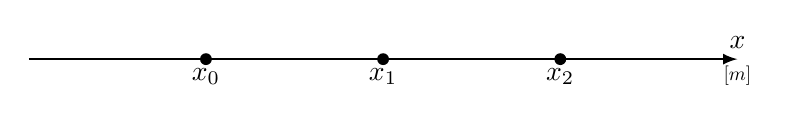
\begin{tikzpicture}[scale=1.5]
   \draw[->,thick,-latex] (-1.75,0) -- (4.25,0) node [anchor=north ,scale=0.7] {$[\text{m}]$}node [anchor=south ,scale=1] {$x $}; 
     \fill[black] (-0.25,0) circle (0.5mm) node [anchor=north ,scale=1] {$x_0$};
   \fill[black] (1.25,0) circle (0.5mm) node [anchor=north ,scale=1] {$x_1$};
    \fill[black] (2.75,0) circle (0.5mm) node [anchor=north ,scale=1] {$x_{2}$};
   
   \end{tikzpicture}
   $$
   A sum of values is known as a series.  Series may be represented using sigma notation.
$$x_0+x_1+x_2 \dots x_M=\sum_{i=0}^{M}x_i$$

\marginnote[-90pt]{$\braket{x}$ is the mean, or average value of a set.  $\sigma$ is the uncertainty or standard deviation.
$$\braket{x}=\frac{x_0+x_1+x_2 \dots}{N}$$
$$\braket{x^2}=\frac{x_0^2+x_1^2+x_2^2 \dots}{N}$$
$$\sigma^2= \braket{x^2}-\braket{x}^2$$
}
  
\section{Difference} 
The delta operator $\Delta$ indicates difference.  $\Delta x$ is a change in $x$ from $x=a$ to $x=b$.
$\Delta x = b-a$, or indexed $\Delta x_i = x_{i+1}-x_i$.
$$\{ \Delta x_i\}=\{x_1 -x_0,x_2-x_1,\dots ,x_N-x_{N-1}\}$$
 

\marginnote[-50pt]{For any sequence $x_i$ with $N$ elements we can generate a sequence $\Delta x_i$ of changes.  This is a mapping of one sequence to another.\\ \  \\
\texttt{
for (i=0,i<N-1,i=i+1)\\
\ \ \ \ \ dx[i]=x[i+1]-x[i]
	}\\ 
	\Large $$\{x_i\}\xrightarrow{\ \ \Delta \ \ }\{ \Delta x_i\}$$
}
$$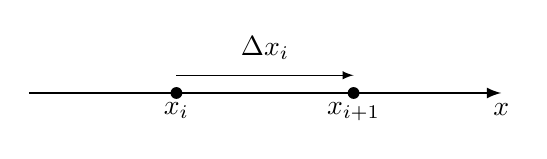
\begin{tikzpicture}[scale=1.5]
   \draw[->,thick,-latex] (0,0) -- (4,0) node [anchor=north ,scale=1] {$x$}; 
      \draw[->,-latex] (1.25,0.15) -- (2.75,0.15)  node [black,midway,above=0pt,yshift=2pt] { $\Delta x_i$}; 
   \fill[black] (1.25,0) circle (0.5mm) node [anchor=north ,scale=1] {$x_i$};
    \fill[black] (2.75,0) circle (0.5mm) node [anchor=north ,scale=1] {$x_{i+1}$};
   
   \end{tikzpicture}
   $$

\section{Accumulation}
Accumulation is the inverse of difference.  Rather than subtract successive terms we add them.  It is the summation of a sequence as a series.  The summation of $\Delta x_i$ returns us to the sequence $x_i$.
\marginnote[-25pt]{For any sequence $\Delta x_i$ of changes we can generate a sequence $x_i$ (up to a constant).  This is the reverse mapping.\\ \ \\ \ \\ \ \\
\texttt{for (i=0,i<N-1,i=i+1)\\
\ \ \ \ \ x[i+1]=x[i]+dx[i]
	}\\ \ \\
	\Large$$\{\Delta x_i\}\xrightarrow{\ \ \sum \ \ }\{  x_i\}$$
}

$$\sum_{n=0}^{i-1}\Delta x_n=x_i-x_0$$
$$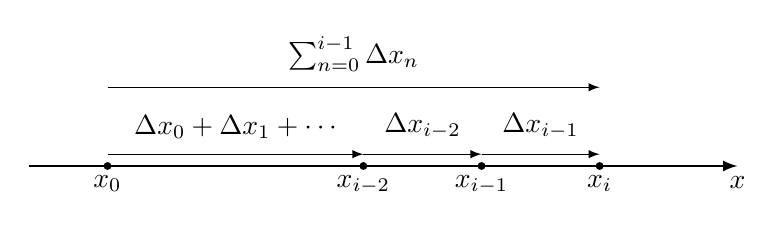
\begin{tikzpicture}[scale=1]
   \draw[->,thick,-latex] (-3,0) -- (6,0) node [anchor=north ,scale=1] {$x$}; 
      \draw[->,-latex] (-2,0.15) -- (1.25,0.15)  node [black,midway,above=0pt,yshift=2pt] { $\Delta x_{0}+\Delta x_{1}+\cdots$}; 
        \draw[->,-latex] (1.25,0.15) -- (2.75,0.15)  node [black,midway,above=0pt,yshift=2pt] { $\Delta x_{i-2}$}; 
          \draw[->,-latex] (2.75,0.15) -- (4.25,0.15)  node [black,midway,above=0pt,yshift=2pt] { $\Delta x_{i-1}$}; 
       \fill[black] (-2,0) circle (0.5mm) node [anchor=north ,scale=1] {$x_0$};
   \fill[black] (1.25,0) circle (0.5mm) node [anchor=north ,scale=1] {$x_{i-2}$};
    \fill[black] (2.75,0) circle (0.5mm) node [anchor=north ,scale=1] {$x_{i-1}$};
     \fill[black] (4.25,0) circle (0.5mm) node [anchor=north ,scale=1] {$x_{i}$};
     \draw[->,-latex] (-2,1) -- (4.25,1)  node [black,midway,above=0pt,yshift=2pt] { $\sum_{n=0}^{i-1}\Delta x_n$}; 

   
   \end{tikzpicture}
   $$

  
\section{Functions}
Given a sequence of discrete ordered pairs $\{x_i,y_i\}$ we can graph points on a 2-dimensional graph using two number lines.  We can model the relationship using a continuous function, $y=f(x)$.
\begin{figure}
$$
\begin{tikzpicture}
      [yscale=0.8, xscale=0.8,line cap=round,line join=round,x=2cm,y=2cm]%main layer

%main layer
%creating the ticks and xy-axis nodes
  \draw[-latex,color=black,thin] (-0.4,0) -- (2.8,0) node [anchor=north ,scale=1] {$x$};
   \draw[-latex,color=black,thin] (0,-0.4) -- (0,1.5)node [anchor=east ,scale=1] {$y$};
 \draw (0.5,1.2) node [anchor=west ,scale=1] {$\{x_i,y_i\}$};
%some function


 
\foreach \x in {-4,...,26}
                             \draw[fill] (\x*0.1,{1/2*(\x*.1) ^2-1/24*(\x*.1)^4+rand*0.1}) circle [radius=.5pt];

\begin{scope}[shift={(3.5,0)}]

  \draw[-latex,color=black,thin] (-0.4,0) -- (2.8,0) node [anchor=north ,scale=1] {$x$};
   \draw[-latex,color=black,thin] (0,-0.4) -- (0,1.5)node [anchor=east ,scale=1] {$y$};
    \draw (0.5,1.2) node [anchor=west ,scale=1] {$f(x)$};

%some function

 \draw[smooth,samples=100,domain=-0.4:2.6]
                             plot(\x,{1/2*(\x) ^2-1/24*(\x)^4});
 
\end{scope}

\end{tikzpicture}
$$

\caption{Ordered pairs $\{x_i,y_i\}$ and continuous function $f(x)$}
  \label{fig:function}
\end{figure}


\begin{figure}
$$
\begin{tikzpicture}
      [yscale=0.8, xscale=0.8,line cap=round,line join=round,x=2cm,y=2cm]%main layer

%main layer
%creating the ticks and xy-axis nodes
  \draw[-latex,color=black,thin] (-0.4,0) -- (2.8,0) node [anchor=north ,scale=1] {$x$};
   \draw[-latex,color=black,thin] (0,-0.4) -- (0,1.5)node [anchor=east ,scale=1] {$y$};
    \draw (0.6,1.2) node [anchor=west ,scale=1] {$\sin (x) $};
    \draw (0.6,-0.6) node [anchor=west ,scale=1] {$\cos (x) $};

%some function

 \draw[smooth,samples=100,domain=-0.4:2.6]
                             plot(\x,cos(90* \x));
                             
  \draw[smooth,samples=100,domain=-0.4:2.6]
                             plot(\x,sin(90* \x));
 
 
\begin{scope}[shift={(0,2.5)}]
%main layer
%creating the ticks and xy-axis nodes
  \draw[-latex,color=black,thin] (-0.4,0) -- (2.8,0) node [anchor=north ,scale=1] {$x$};
   \draw[-latex,color=black,thin] (0,-0.4) -- (0,1.5)node [anchor=east ,scale=1] {$y$};
    \draw (0.75,1.3) node [anchor=west ,scale=1] {$\sqrt{x}$};
    \draw (0.75,0.45) node [anchor=west ,scale=1] {$\nicefrac{1}{x}$};

%some function

 \draw[smooth,samples=100,domain=0.15:2.6]
                             plot(\x,0.2/\x);
                             
  \draw[smooth,samples=100,domain=0:2.6]
                             plot(\x,sqrt \x);
 \end{scope}
 
 
\begin{scope}[shift={(-3.5,2.5)}]
%main layer
%creating the ticks and xy-axis nodes
  \draw[-latex,color=black,thin] (-0.4,0) -- (2.8,0) node [anchor=north ,scale=1] {$x$};
   \draw[-latex,color=black,thin] (0,-0.4) -- (0,1.5)node [anchor=east ,scale=1] {$y$};
    \draw (0.75,1.2) node [anchor=west ,scale=1] {$mx+b$};
    \draw (0.6,0.2) node [anchor=west ,scale=1] {$ax^2+bx+c$};

%some function

 \draw[smooth,samples=100,domain=-0.4:2.6]
                             plot(\x,\x*.4+0.3);
                             
  \draw[smooth,samples=100,domain=-0.4:2.6]
                             plot(\x,\x*\x*0.33-.8*\x+.3);
 \end{scope}
 
 \begin{scope}[shift={(-3.5,0)}]
%main layer
%creating the ticks and xy-axis nodes
  \draw[-latex,color=black,thin] (-0.4,0) -- (2.8,0) node [anchor=north ,scale=1] {$x$};
   \draw[-latex,color=black,thin] (0,-0.4) -- (0,1.5)node [anchor=east ,scale=1] {$y$};
    \draw (0.75,1.2) node [anchor=west ,scale=1] {$e^x$};
    \draw (0.75,-0.6) node [anchor=west ,scale=1] {$\log(x) $};

%some function

 \draw[smooth,samples=100,domain=-0.4:2]
                             plot(\x,0.3*exp (\x*0.8) );
                             
  \draw[smooth,samples=100,domain=0.5:2.6]
                             plot(\x,ln \x);
 \end{scope}
 
\end{tikzpicture}
$$
\caption{Common functions}
  \label{fig:function}
\end{figure}
\begin{margintable}[-300pt]
\begin{center}
\footnotesize
\begin{tabular}{lllll}
\toprule
 Function              & Formula                                                                         \\
\midrule
  Linear   & $y=mx+b$       \\
  Quadratic  & $y=ax^2+bx+c$           \\
    Reciprocal    & $y=\frac{1}{x}$                        \\
    Power         & $y=x^n$                                                        \\
    Exponential        & $y=a^x$                              \\
    Logarithmic          & $y=\log_a b$          \\
     Sine         & $y=\sin x$                                                        \\
    Cosine       & $y=\cos x$                              \\
    Tangent        & $y=\tan x$          \\
  Arc sine         & $y=\sin^{-1} x$                                                        \\
    Arc cosine       & $y=\cos^{-1} x$                              \\
    Arc tangent        & $y=\tan^{-1} x$          \\
\bottomrule
\end{tabular}
\end{center}
  \caption{A list of common functions}
  \label{tab:font-sizes}
\end{margintable}

\subsection{Changing Functions}
\newthought{Changes in the value of a function} generate difference in $f(x)$.  There is a relationship between $\Delta f$ and $\Delta x$.
\begin{fullwidth}
\begin{figure}[h]
$$
\definecolor{darkgray}{rgb}{0.25,0.25,0.25}
\definecolor{lightgray}{rgb}{0.75,0.75,0.75}
%
\definecolor{darkgray}{rgb}{0.25,0.25,0.25}
\definecolor{lightgray}{rgb}{0.75,0.75,0.75}
%
\begin{tikzpicture}
      [yscale=1.3, xscale=3.3,line cap=round,line join=round,x=2cm,y=2cm,
     %using the 'spy' to magnify a part of the picture
     spy using outlines={rectangle,lens={scale=3}, size=4.5cm, connect spies},
     %using the decoration 'brace' (=a curly brace as path replacement)
     decoration={brace,amplitude=2pt}]%main layer

%main layer
%creating the ticks and xy-axis nodes
  \draw[-latex,color=black,thin] (-0.2,0) -- (1.4,0) node [anchor=north ,scale=1] {$x$};
   \draw[-latex,color=black,thin] (0,-0.2) -- (0,1.4)node [anchor=east ,scale=1] {$y$};
    \draw (1,1) node [anchor=west ,scale=1] {$f(x)$};
 
%some function

 \draw[smooth,samples=100,domain=-0.2:1.3]
                             plot(\x,{1/2*(\x*2) ^2-1/24*(\x*2)^4});
 
  \draw [darkgray,ultra thin] (0,0.1224)-- (0.25,0.1224);
  \draw [darkgray,ultra thin] (0,0.914)-- (0.75,0.914);
  \draw [darkgray,ultra thin] (0.25,0.1224)-- (0.25,0.0);
  \draw [darkgray,ultra thin] (0.75,0.914)-- (0.75,0);
%creating the curly braces with decorate
  \draw [decorate,color=black] (-0.01,0.1224) -- (-0.01,0.914) 
   node [midway,anchor=east,inner sep=2pt, outer sep=1pt]{\small$\Delta f$};
  \draw [decorate,color=black!80!black] (0.75,-0.02) -- (0.25,-0.02)
   node [midway,anchor=north,inner sep=1pt, outer sep=1pt]{\small$\Delta x$};
    \draw (0.75,-0.05)  node [anchor=north ,scale=0.75] {$b$};
     \draw (.25,-0.05) node [anchor=north ,scale=0.75] {$a$};
      \draw (0,0.1224)  node [anchor=east ,scale=0.75] {$f(a) \ $};
     \draw (0,0.914) node [anchor=east ,scale=0.75] {$f(b) \ $};
\end{tikzpicture}
$$

\caption{Difference on a continuous function $f(x)$}
  \label{fig:function-delta}
\end{figure}
\end{fullwidth}
\vspace{0.5cm}
\marginnote[0pt]{\textit{Difference is the object of a practical affirmation inseparable from essence and constitutive of existence.}\textbf{- Gilles Deleuze}}
$$\Delta f= f(b)-f(a)$$
$$\Delta f= f(a+\Delta x)-f(a)$$


\newpage

\subsection{Slope, Tangent Line \& Slope Function }
The \textbf{slope} is a ratio of difference between two points on the function graph.  The construction of the right triangle with sides $\Delta x$ and $\Delta y$ yields a tangent which is equivalent to the slope.  In the limit of small $\Delta$ we call the slope a \textbf{tangent line}.
\begin{figure}[ht]
$$\definecolor{darkgray}{rgb}{0.25,0.25,0.25}
\definecolor{lightgray}{rgb}{0.75,0.75,0.75}
%
\definecolor{darkgray}{rgb}{0.25,0.25,0.25}
\definecolor{lightgray}{rgb}{0.75,0.75,0.75}
%
\begin{tikzpicture}
   [xscale=2,line cap=round,line join=round,x=2cm,y=2cm,
     %using the 'spy' to magnify a part of the picture
     spy using outlines={rectangle,lens={scale=2}, size=4cm, connect spies},
     %using the decoration 'brace' (=a curly brace as path replacement)
     decoration={brace,amplitude=2pt}]%main layer
%creating the ticks and xy-axis nodes
  \draw[-latex,color=black,thin] (-0.2,0) -- (1.4,0) node [anchor=north ,scale=1] {$x$};
   \draw[-latex,color=black,thin] (0,-0.2) -- (0,1.4)node [anchor=east ,scale=1] {$y$};
    \draw (1,1) node [anchor=west ,scale=1] {$f(x)$};
 
%some function

 \draw[smooth,samples=100,domain=0.0:1.3]
                             plot(\x,{1/2*(\x*2) ^2-1/24*(\x*2)^4});
 
  \draw [darkgray,ultra thin] (0,0.1224)-- (0.25,0.1224);
  \draw [darkgray,ultra thin] (0,0.235)-- (0.35,0.235);
  \draw [darkgray,ultra thin] (0.25,0.1224)-- (0.25,0.0);
  \draw [darkgray,ultra thin] (0.35,0.235)-- (0.35,0);
%creating the curly braces with decorate
  \draw [decorate,color=black] (-0.01,0.1224) -- (-0.01,0.235)
   node [midway,anchor=east,inner sep=2pt, outer sep=1pt]{\tiny$\Delta f $};
  \draw [decorate,color=black!80!black] (0.35,-0.01)--(0.25,-0.01)
   node [midway,anchor=north,inner sep=1pt, outer sep=2pt]{\tiny$ \Delta x$};
   
    \draw[smooth,color=red, samples=100,domain=0.05:0.5]
                             plot(\x,{((0.235-0.1224)/0.1)*(\x-0.25)+0.122});

   
   \spy [blue!50] on (0.275,0.3)
             in node [left] at (2.5,0.7);
             
                \draw (2.5,0.7) node [anchor=south east,color=red ,scale=1] {slope$=\frac{\Delta f}{\Delta x}$};
\end{tikzpicture}
$$\\ \ \\ 
$$\definecolor{darkgray}{rgb}{0.25,0.25,0.25}
\definecolor{lightgray}{rgb}{0.75,0.75,0.75}
%
\definecolor{darkgray}{rgb}{0.25,0.25,0.25}
\definecolor{lightgray}{rgb}{0.75,0.75,0.75}
%
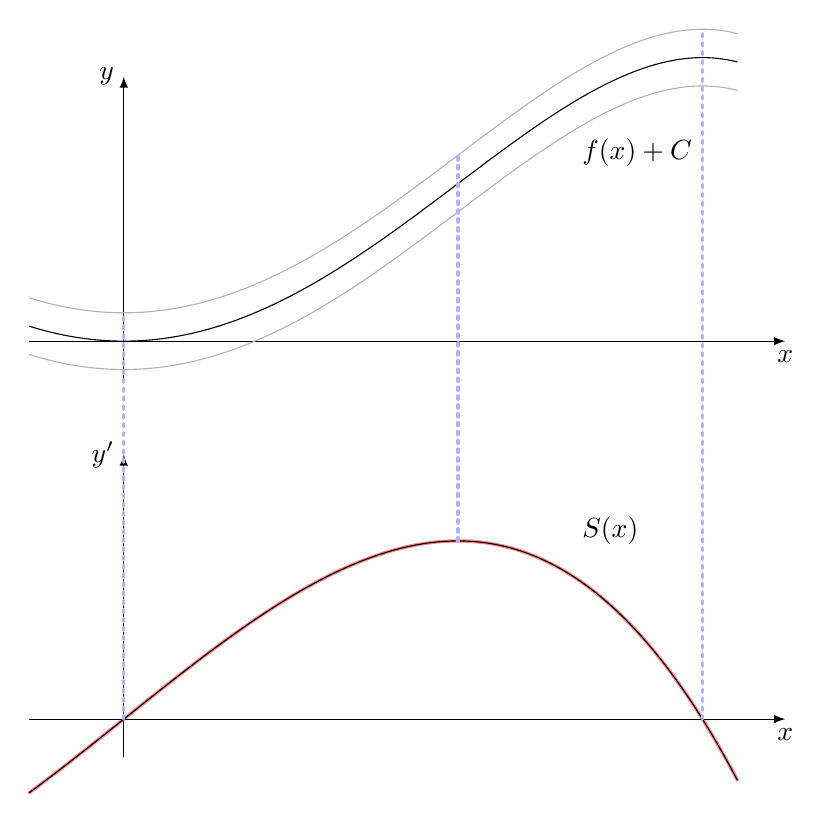
\begin{tikzpicture}
      [line cap=round,line join=round,x=2cm,y=2cm, yscale=1.2, xscale=3]
   

%main layer
%creating the ticks and xy-axis nodes
  \draw[-latex,color=black,thin] (-0.2,0) -- (1.4,0) node [anchor=north ,scale=1] {$x$};
   \draw[-latex,color=black,thin] (0,-0.2) -- (0,1.4)node [anchor=east ,scale=1] {$y$};
    \draw (0.95,1) node [anchor=west ,scale=1] {$f(x)+C$};
 
%some function

 \draw[smooth,samples=100,domain=-0.2:1.3] plot(\x,{1/2*(\x*2) ^2-1/24*(\x*2)^4});
  \draw[smooth,samples=100,domain=-0.2:1.3,color=black!30] plot(\x,{1/2*(\x*2) ^2-1/24*(\x*2)^4-0.15});
   \draw[smooth,samples=100,domain=-0.2:1.3,color=black!30] plot(\x,{1/2*(\x*2) ^2-1/24*(\x*2)^4+0.15});
 
 \begin{scope}[shift={(0,-2)}]
 	\draw[smooth,samples=100,domain=-0.2:1.3,color=red!50, very thick] plot(\x,{(\x*2)-1/6*(\x*2)^3});            
	\draw[smooth,samples=100,domain=-0.2:1.3,thin] plot(\x,{(\x*2)-1/6*(\x*2)^3});                   
	       
	\draw[-latex,color=black,thin] (-0.2,0) -- (1.4,0) node [anchor=north ,scale=1] {$x$};
	\draw[-latex,color=black,thin] (0,-0.2) -- (0,1.4)node [anchor=east ,scale=1] {$y'$};
	\draw (0.95,1) node [anchor=west ,scale=1] {$S(x)$};
 \end{scope}
 
 \draw[dotted,color=blue!30, very thick] (1.225,-2) -- (1.225,1.65);
 \draw[dotted,color=blue!30, very thick] (0,-2) -- (0,0.15);
 \draw[dotted,color=blue!30,very thick] (0.707,-1.057) -- (0.707,0.983);
 
\end{tikzpicture}$$

\caption{Tangent lines and the slope function S(x) for a function $f(x)$}
  \label{fig:function-delta}
\end{figure}

\marginnote[-260pt]{
This specific function $f(x)$ is 
$$y=x^2-\frac{x^4}{12}$$}

\marginnote[-450pt]{
\Large $$\text{slope}=\frac{\text{rise}}{\text{run}}=\frac{\Delta f}{\Delta x}$$}

\marginnote[-130pt]{
$$S(x)=\text{slope of tangent line}=\mathop {\lim }\limits_{\Delta x \to 0} {\frac{\Delta f}{\Delta x}}$$\\ \ \\
This specific slope function $S(x)$ is \\ \ \\
$$y=2x-\frac{x^3}{3}$$
}

\noindent The \textbf{slope function} $S(x)$ represents the slope of the tangent line at any point $x$.


\newpage


\subsection{Accumulation of a Slope Function}
Over some range $\Delta x$ the area beneath the slope function represents some accumulation of $S(x)$.  The total area represents $\Delta f$  over the range $\Delta x$.
\begin{figure}[ht]
$$\definecolor{darkgray}{rgb}{0.25,0.25,0.25}
\definecolor{lightgray}{rgb}{0.75,0.75,0.75}
%
\definecolor{darkgray}{rgb}{0.25,0.25,0.25}
\definecolor{lightgray}{rgb}{0.75,0.75,0.75}
%
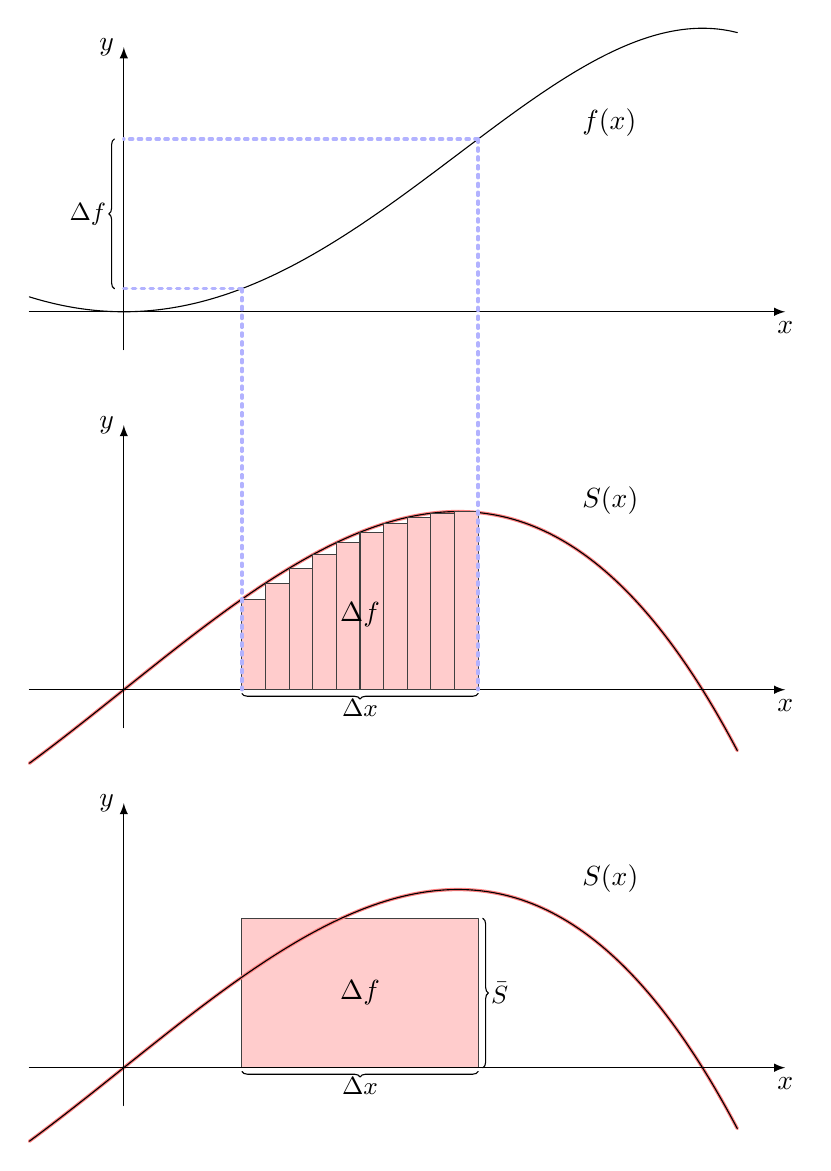
\begin{tikzpicture}
      [line cap=round,decoration={brace,amplitude=2pt},line join=round,x=2cm,y=2cm, yscale=1.2, xscale=3]
   

%main layer
%creating the ticks and xy-axis nodes
  \draw[-latex,color=black,thin] (-0.2,0) -- (1.4,0) node [anchor=north ,scale=1] {$x$};
   \draw[-latex,color=black,thin] (0,-0.2) -- (0,1.4)node [anchor=east ,scale=1] {$y$};
    \draw (0.95,1) node [anchor=west ,scale=1] {$f(x)$};
 
%some function

 \draw[smooth,samples=100,domain=-0.2:1.3] plot(\x,{1/2*(\x*2) ^2-1/24*(\x*2)^4});
 
 
 \begin{scope}[shift={(0,-2)}]
 	\draw[smooth,samples=100,domain=-0.2:1.3,color=red!50, very thick] plot(\x,{(\x*2)-1/6*(\x*2)^3});            
	\draw[smooth,samples=100,domain=-0.2:1.3,thin] plot(\x,{(\x*2)-1/6*(\x*2)^3});                   
	       
	\draw[-latex,color=black,thin] (-0.2,0) -- (1.4,0) node [anchor=north ,scale=1] {$x$};
	\draw[-latex,color=black,thin] (0,-0.2) -- (0,1.4)node [anchor=east ,scale=1] {$y$};
	\draw (0.95,1) node [anchor=west ,scale=1] {$S(x)$};
	
	 \foreach \x in {0.25,0.3,0.35,0.4,0.45,0.5,0.55,0.6,0.65,0.7}
   \fill[color=red!20,thin] (\x,0) -- (\x,{(\x*2)-1/6*(\x*2)^3}) -- (\x+0.05,{(\x*2)-1/6*(\x*2)^3}) -- (\x+0.05,0) -- cycle;
   \foreach \x in {0.25,0.3,0.35,0.4,0.45,0.5,0.55,0.6,0.65,0.7}
   \draw[color=darkgray,thin] (\x,0) -- (\x,{(\x*2)-1/6*(\x*2)^3}) -- (\x+0.05,{(\x*2)-1/6*(\x*2)^3}) -- (\x+0.05,0) -- cycle;

  \draw [decorate,color=black!80!black] (0.75,-0.02) -- (0.25,-0.02)
   node [midway,anchor=north,inner sep=1pt, outer sep=1pt]{\small$\Delta x$};
    \draw (0.5,0.4)
   node [anchor=center,scale=1]{$\Delta f$};
 \end{scope}
 
 \draw[dotted,color=blue!30, very thick] (0.25,0.1224) -- (0,0.1224);
 \draw[dotted,color=blue!30, very thick] (0.75,0.914) -- (0,0.914);
 \draw[dotted,color=blue!30, very thick] (0.25,0.1224) -- (0.25,-2);
 \draw[dotted,color=blue!30, very thick] (0.75,0.914) -- (0.75,-2);

 
   \draw [decorate,color=black] (-0.02,0.1224) -- (-0.02,0.914) 
   node [midway,anchor=east,inner sep=2pt, outer sep=1pt]{\small$\Delta f$};
  
   \begin{scope}[shift={(0,-4)}]
   \fill[color=red!20,thin] (0.25,0) -- (0.25,0.79) -- (0.75,0.79) -- (0.75,0) -- cycle;
   \draw[color=darkgray,thin] (0.25,0) -- (0.25,0.79) -- (0.75,0.79) -- (0.75,0) -- cycle;
 	\draw[smooth,samples=100,domain=-0.2:1.3,color=red!50, very thick] plot(\x,{(\x*2)-1/6*(\x*2)^3});            
	\draw[smooth,samples=100,domain=-0.2:1.3,thin] plot(\x,{(\x*2)-1/6*(\x*2)^3});                   
	       
	\draw[-latex,color=black,thin] (-0.2,0) -- (1.4,0) node [anchor=north ,scale=1] {$x$};
	\draw[-latex,color=black,thin] (0,-0.2) -- (0,1.4)node [anchor=east ,scale=1] {$y$};
	\draw (0.95,1) node [anchor=west ,scale=1] {$S(x)$};

  \draw [decorate,color=black!80!black] (0.75,-0.02) -- (0.25,-0.02)
   node [midway,anchor=north,inner sep=1pt, outer sep=1pt]{\small$\Delta x$};
   
     \draw [decorate,color=black] (0.76,0.79) -- (0.76,0) 
   node [midway,anchor=west,inner sep=2pt, outer sep=1pt]{\small$\bar{S}$};
   
   \draw (0.5,0.4) node [anchor=center ,scale=1] {$\small\Delta f$};
   
 \end{scope}
  
\end{tikzpicture}$$
\caption{Area underneath a slope function $S(x)$}
  \label{fig:functiona-delta}
\end{figure}

\marginnote[-140pt]{
 \Large $$\bar{S}=\frac{\Delta f}{\Delta x}$$\\
 
 \Large  $$\Delta f=\bar{S}\cdot {\Delta x}$$
   }
   \noindent If this area representing $\Delta f$ is represented as a rectangle with base $\Delta x$ the height of the rectangle is the average value $\bar{S}$.
\newpage


\section{Scalars and Vectors}
A \textbf{scalar} is a one-dimensional physical quantity, i.e. one that can be described by a single real number (signed, with units).  It is a physical quantity that only has magnitude but no direction.  A \textbf{vector} is a geometric object that has magnitude (or length) and direction and can be added to other vectors according to vector algebra.  A vector can be represented by a set of scalars.  

$\overrightarrow{x}$ is a vector.  $x$ is the magnitude (or length) of the vector $\overrightarrow{x}$.  The vector $\hat{x}$ is the directional vector of $\overrightarrow{x}$.  It has a magnitude of 1 rand points in the same direction as $\overrightarrow{x}$.  
\marginnote[-100pt]{ \Large
$$\overrightarrow{x}=x\hat{x}$$\\ \ \\
$$|\overrightarrow{x}|=x$$\\ \ \\
$$\hat{x}=\frac{\overrightarrow{x}}{x}$$\\ \ \\
$$|\hat{x}|=1$$
}
$$
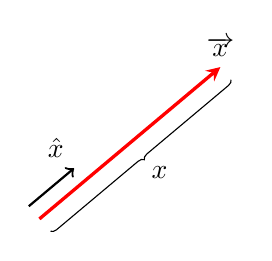
\begin{tikzpicture}[scale=3,decoration={brace,amplitude=2pt}]



%draw a vector from origin to point (P) 
\begin{scope}[rotate=40]
\draw[-stealth,very thick,color=red] (0,0) -- (1,0) node[anchor=south,color=black]{$\overrightarrow{x}$};
  \draw[->,thick,color=black] (0,0.07) -- (0.25,0.07) node[anchor=south east,color=black]{$\hat{x}$};
   \draw [decorate,color=black] (1,-0.07) -- (0,-0.07) 
   node [midway,anchor=north west,inner sep=2pt, outer sep=2pt]{$x$};
   \end{scope}



\end{tikzpicture}
$$

\section{Spatial Coordinate Systems}
\subsection{2D Cartesian $(x,y)$}


In two dimensions we use the vector representation $\overrightarrow{r}$ with components $x$ and $y$.  This can be represented as a column vector or using the unit vectors $\hat{x}$ and $\hat{y}$.  The magnitude of the vector $\overrightarrow{r}$ is $r$.  We can calculate $r$ given the $x$ and $y$ components using the Pythagorean theorem.

$x$ (or $r_x$) and $y$ (or $r_y$) are called orthogonal components of $\overrightarrow{r}$ meaning $\hat{x}$ and $\hat{y}$ do not overlap at all, namely they meet at 90 degrees.

\marginnote[-20pt]{\Large
$$\overrightarrow{r}=x\hat{x}+y\hat{y}$$\\ \ \\
$$ \overrightarrow{r}=\left(\begin{array}{c} x \\ y \end{array}\right)$$\\ \ \\
$$r=\sqrt{x^2+y^2}$$\\ \ \\
$$\hat{r}=\left(\begin{array}{c} \nicefrac{x}{\sqrt{x^2+y^2}} \\ \nicefrac{y}{\sqrt{x^2+y^2}} \end{array}\right)$$
}
\vspace{1cm}
$$
\begin{tikzpicture}[scale=1.5]


\draw[thick,->] (0,0,0) -- (3,0,0) node[anchor=north east]{$x$};
\draw[thick,->] (0,0,0) -- (0,3,0) node[anchor=north west]{$y$};


%draw a vector from origin to point (P) 
\draw[-stealth,very thick,color=red] (0,0) -- (1,2) node[anchor=south west,color=black]{$\overrightarrow{r}$};


%draw projection on xy plane, and a connecting line
\draw[dashed, color=red] (1,0) -- (1,2) node[midway,anchor=west ,scale=1,color=black] {$r_y$};
\draw[dashed, color=red] (0,2) -- (1,2) node[midway,anchor=south ,scale=1,color=black] {$r_x$};
\end{tikzpicture}
$$
\newpage
\subsection{Polar Coordinates $(r,\theta)$ }
In polar coordinates we parameterize the vector $\overrightarrow{r}$ in terms of its length and direction rather than in terms of the $x$ and $y$ components.  The length of the vector $\overrightarrow{r}$ is $r$ and the direction is expressed in terms of $\theta$.  The vector $\overrightarrow{r}$ makes an angle $\theta$ with the unit vector $\hat{x}$.  We can easily convert between polar coordinates $(r,\theta)$ and 2-D cartesian coordinates $(x,y)$. 

\marginnote[-80pt]{\Large

$$\overrightarrow{r}=r\hat{r}$$\\ \ \\
$$r=\sqrt{x^2+y^2}$$\\ \ \\
$$\theta=\tan^{-1}\left(\frac{y}{x}\right)$$\\ \ \\
$$x=r\cos\theta$$\\ \ \\
$$y=r\sin\theta$$\\ \ \\
$$\hat{r}=\left(\begin{array}{c} \cos \theta \\ \sin \theta \end{array}\right)$$\\ \ \\ \ \\

\footnotesize
In mathematics, the polar coordinate system is a two-dimensional coordinate system in which each point on a plane is determined by a distance from a reference point and an angle from a reference direction.\\ 

The reference point (analogous to the origin of a Cartesian system) is called the pole, and the ray from the pole in the reference direction is the polar axis. The distance from the pole is called the radial coordinate or radius, and the angle is the angular coordinate, polar angle, or azimuth.\\ 

The concepts of angle and radius were already used by ancient peoples of the 1st millennium BC. The Greek astronomer and astrologer Hipparchus (190-120 BC) created a table of chord functions giving the length of the chord for each angle, and there are references to his using polar coordinates in establishing stellar positions. In On Spirals, Archimedes describes the Archimedean spiral, a function whose radius depends on the angle. The Greek work, however, did not extend to a full coordinate system.}

\vspace{1cm}
$$
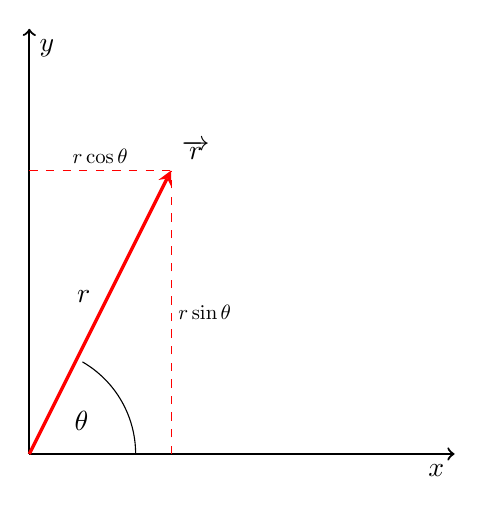
\begin{tikzpicture}[scale=1.8]


\draw[thick,->] (0,0,0) -- (3,0,0) node[anchor=north east]{$x$};
\draw[thick,->] (0,0,0) -- (0,3,0) node[anchor=north west]{$y$};


%draw a vector from origin to point (P) 
\draw[-stealth,very thick,color=red] (0,0) -- (1,2) node[anchor=south west,color=black]{$\overrightarrow{r}$};
\draw[color=red] (0,0) -- (0.5,1) node[anchor=south east ,color=black]{$r$};
\draw[dashed, color=red] (1,0) -- (1,2) node[midway,anchor=west ,scale=0.75,color=black] {$r\sin \theta$};
\draw[dashed, color=red] (0,2) -- (1,2) node[midway,anchor=south ,scale=0.75,color=black] {$r \cos \theta$};


%draw projection on xy plane, and a connecting line
\draw (0.75,0) arc (0:60:0.75) ;
\draw (0.25,0.1) node [anchor=south west,color=black]{$\theta$};
\end{tikzpicture}
$$
\vspace{1cm}
$$
  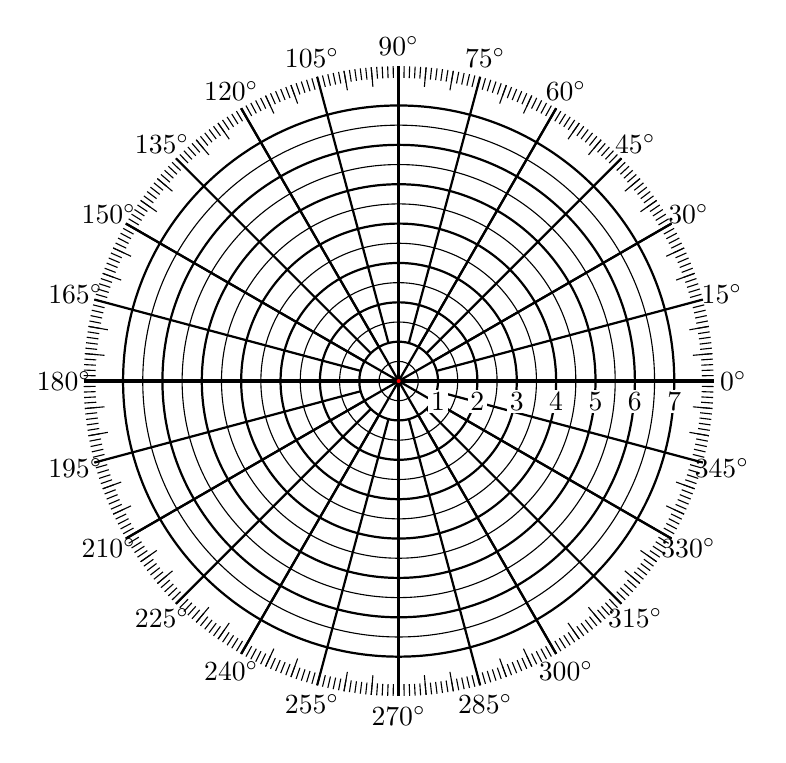
\begin{tikzpicture} [yscale=0.5, xscale=0.5]
    %Circles 
    \foreach \r in {1, 2,...,7}
      \draw[ thick] (0,0) circle (\r);    
    \foreach \r in {0.5, 1.5,...,7}
      \draw[thin] (0,0) circle (\r);
    %1� Rays
    \foreach \a in {0, 1,...,359}
      \draw[] (\a:7.7) -- (\a:8);
    %5� Rays
    \foreach \a in {0, 5,...,359}
      \draw[] (\a:7.5) -- (\a:8);      
    %15� Rays
    \foreach \a in {0, 15,...,359}
      \draw[thick] (\a:1) -- (\a:8); 
    %30� Rays
    \foreach \a in {0, 30,...,359}
      \draw[thick] (0, 0) -- (\a:8);
    %Radius labels (background filled white)
    \foreach \r in {1, 2,...,7}
      \draw (\r,0) node[inner sep=1pt,below=3pt,rectangle,fill=white] {$\r$};
    %Main rays
    \foreach \a in {0, 90,...,359}
      \draw[very thick] (0, 0) -- (\a:8);
    %Angle labels  
    \foreach \a in {0, 15,...,359}
      \draw (\a: 8.5) node {$\a^\circ$};
    %Central point
    \draw[fill=red] (0,0) circle(0.7mm);
  \end{tikzpicture}
$$

\newpage

\subsection{3D Cartesian $(x,y,z)$}
\marginnote[0pt]{
In three dimensions a vector can be described by three orthogonal components $(x,y,z)$.  It is the 3D cartesian coordinate system.  These form a right handed coordinate system so that if you look at the standard $(x,y)$ plane the z-axis comes straight out of the page.  The magnitude of $\overrightarrow{\scriptr}$ is determined using the Pythagorean Theorem (in 3D).\\
$$\scriptr=\sqrt{x^2+y^2+z^2}$$\\



The concept of Cartesian coordinates generalizes to allow axes that are not perpendicular to each other, and/or different units along each axis. In that case, each coordinate is obtained by projecting the point onto one axis along a direction that is parallel to the other axis (or, in general, to the hyperplane defined by all the other axes). In such an oblique coordinate system the computations of distances and angles must be modified from that in standard Cartesian systems, and many standard formulas (such as the Pythagorean formula for the distance) do not hold.\\ \ \\

We use the $\overrightarrow{\scriptr}$ to notate the vector in 3D and reserve $\overrightarrow{r}$ to represent the component in the xy-plane.  In cylindrical coordinates the vector $\overrightarrow{\scriptr}$ is represented using polar coordinates for  $\overrightarrow{r}$ and an orthogonal z-component.  Converting between cylindrical and 3D cartesian coordinates is identical to the polar and 2D cartesian conversion.}
\vspace{1cm}
$$\overrightarrow{\scriptr}=\overrightarrow{x}+\overrightarrow{y}+\overrightarrow{z}=x\hat{x}+y\hat{y}+z\hat{z}=\scriptr_x\hat{x}+\scriptr_y\hat{y}+\scriptr_z\hat{z}$$
$$ \overrightarrow{\scriptr}=\left(\begin{array}{c} x \\ y \\ z\end{array}\right)=\left(\begin{array}{c} \scriptr_x \\ \scriptr_y \\ \scriptr_z\end{array}\right)$$

\tdplotsetmaincoords{60}{110}
\begin{tikzpicture}[scale=1.2,tdplot_main_coords]
\coordinate (O) at (0,0,0);
\coordinate (P) at (1,2,3);

\draw[thick,->] (0,0,0) -- (4,0,0) node[anchor=north east]{$x$};
\draw[thick,->] (0,0,0) -- (0,4,0) node[anchor=north west]{$y$};
\draw[thick,->] (0,0,0) -- (0,0,4) node[anchor=south]{$z$};

%draw a vector from origin to point (P) 
\draw[-stealth,color=red] (O) -- (P) node[anchor=south,color=black]{$\overrightarrow{\scriptr}$};


%draw projection on xy plane, and a connecting line
\draw[dashed, color=red] (1,0,0) -- (1,2,0);
\draw[dashed, color=red] (0,2,0) -- (1,2,0);
\draw[dashed, color=red] (1,2,3) -- (1,2,0);

\draw (0.5,2,0) node [anchor=west ,scale=1] {$\scriptr_x$};
\draw (1,1,0) node [anchor=north ,scale=1] {$\scriptr_y$};
\draw (1,2,1.5) node [anchor=west ,scale=1] {$\scriptr_z$};

%draw the angle \phi, and label it
%syntax: \tdplotdrawarc[coordinate frame, draw options]{center point}{r}{angle}{label options}{label}
%\tdplotdrawarc{(O)}{0.2}{0}{\phivec}{anchor=north}{$\phi$}


%set the rotated coordinate system so the x'-y' plane lies within the
%"theta plane" of the main coordinate system
%syntax: \tdplotsetthetaplanecoords{\phi}
%\tdplotsetthetaplanecoords{\phivec}

%draw theta arc and label, using rotated coordinate system
%\tdplotdrawarc[tdplot_rotated_coords]{(0,0,0)}{0.5}{0}{\thetavec}{anchor=south west}{$\theta$}

\end{tikzpicture}

\subsection{Cylindrical $(r,\theta,z)$}
$$\overrightarrow{\scriptr}=\overrightarrow{r}+\overrightarrow{z}=r\hat{r}+z\hat{z}=\scriptr_r\hat{r}+\scriptr_z\hat{z}$$






\tdplotsetmaincoords{60}{110}
\begin{tikzpicture}[scale=1.2,tdplot_main_coords]
\coordinate (O) at (0,0,0);
\coordinate (P) at (1,2,3);

\draw[thick,->] (0,0,0) -- (4,0,0) node[anchor=north east]{$x$};
\draw[thick,->] (0,0,0) -- (0,4,0) node[anchor=north west]{$y$};
\draw[thick,->] (0,0,0) -- (0,0,4) node[anchor=south]{$z$};

%draw a vector from origin to point (P) 
\draw[-stealth,thick,color=red] (O) -- (P) node[anchor=south,color=black]{$\overrightarrow{\scriptr}$};


%draw projection on xy plane, and a connecting line

\draw[dashed, color=red] (0,0,0) -- (1,2,0);
\draw[dashed, color=red] (1,2,3) -- (1,2,0);


\draw (0.5,1,0) node [anchor=north ,scale=1] {$\scriptr_r$};
\draw (1,2,1.5) node [anchor=west ,scale=1] {$\scriptr_z$};

%draw the angle \phi, and label it
%syntax: \tdplotdrawarc[coordinate frame, draw options]{center point}{r}{angle}{label options}{label}
\tdplotdrawarc{(O)}{0.8}{0}{60}{anchor=north}{$\theta$}


%set the rotated coordinate system so the x'-y' plane lies within the
%"theta plane" of the main coordinate system
%syntax: \tdplotsetthetaplanecoords{\phi}
%\tdplotsetthetaplanecoords{\phivec}

%draw theta arc and label, using rotated coordinate system
%\tdplotdrawarc[tdplot_rotated_coords]{(0,0,0)}{0.5}{0}{\thetavec}{anchor=south west}{$\theta$}

\end{tikzpicture}
\hspace{1cm}
\tdplotsetmaincoords{60}{110}
\begin{tikzpicture}[scale=1,tdplot_main_coords]
\coordinate (O) at (0,0,0);
\coordinate (P) at (1,2,0);

\draw[thick,->] (0,0,0) -- (4,0,0) node[anchor=north east]{$x$};
\draw[thick,->] (0,0,0) -- (0,4,0) node[anchor=north west]{$y$};
\draw[thick,->] (0,0,0) -- (0,0,4) node[anchor=south]{$z$};

%draw a vector from origin to point (P) 
\draw[-stealth,color=red] (O) -- (P) node[anchor=north,color=black]{$\overrightarrow{r}$};


%draw projection on xy plane, and a connecting line


%draw the angle \phi, and label it
%syntax: \tdplotdrawarc[coordinate frame, draw options]{center point}{r}{angle}{label options}{label}
\tdplotdrawarc{(O)}{0.8}{0}{60}{anchor=north}{$\theta$}


%set the rotated coordinate system so the x'-y' plane lies within the
%"theta plane" of the main coordinate system
%syntax: \tdplotsetthetaplanecoords{\phi}
%\tdplotsetthetaplanecoords{\phivec}

%draw theta arc and label, using rotated coordinate system
%\tdplotdrawarc[tdplot_rotated_coords]{(0,0,0)}{0.5}{0}{\thetavec}{anchor=south west}{$\theta$}

\end{tikzpicture}
\newpage
\subsection{Spherical $(\scriptr,\theta,\phi)$}
\marginnote[0pt]{In a spherical coordinate system we represent the 3D vector $\overrightarrow{\scriptr}$ in terms of its magnitude (length) $\scriptr$, azimuthal angle $\theta$ and polar angle $\phi$.  The conversion between 3D cartesian or cylindrical coordinates and spherical coordinates are given.\\ \ \\ \
$$\hat{\scriptr}=\left(\begin{array}{c}  \sin \phi\ \cos\theta \\  \sin \phi\ \sin\theta \\ \cos \phi  \end{array}\right)$$ \\ \ \\ \ \\
A spherical coordinate system is a coordinate system for three-dimensional space where the position of a point is specified by three numbers: the radial distance of that point from a fixed origin, its polar angle measured from a fixed zenith direction, and the azimuth angle of its orthogonal projection on a reference plane that passes through the origin and is orthogonal to the zenith, measured from a fixed reference direction on that plane.\\ \ \\

The radial distance is also called the radius or radial coordinate. The polar angle may be called co-latitude, zenith angle, normal angle, or inclination angle.\\ \ \\

The mathematics used to describe electron distributions around atoms uses spherical coordinates.  The symmetry features of this mathematics gives rise to the structure of the periodic table.
}



\vspace{1cm}
$$\overrightarrow{\scriptr}=\scriptr \ \hat{\scriptr}$$
\vspace{1cm}
$$\scriptr=\sqrt{x^2+y^2+z^2}$$
$$\theta=\tan^{-1}\left(\frac{y}{x}\right)$$
$$\phi=\tan^{-1}\left(\frac{r}{z}\right)$$


\tdplotsetmaincoords{60}{110}

%define polar coordinates for some vector
%TODO: look into using 3d spherical coordinate system
\pgfmathsetmacro{\rvec}{.8}
\pgfmathsetmacro{\thetavec}{30}
\pgfmathsetmacro{\phivec}{60}

%start tikz picture, and use the tdplot_main_coords style to implement the display 
%coordinate transformation provided by 3dplot
\begin{tikzpicture}[scale=5,tdplot_main_coords]

%set up some coordinates 
%-----------------------
\coordinate (O) at (0,0,0);

%determine a coordinate (P) using (r,\theta,\phi) coordinates.  This command
%also determines (Pxy), (Pxz), and (Pyz): the xy-, xz-, and yz-projections
%of the point (P).
%syntax: \tdplotsetcoord{Coordinate name without parentheses}{r}{\theta}{\phi}
\tdplotsetcoord{P}{\rvec}{\thetavec}{\phivec}

%draw figure contents
%--------------------

%draw the main coordinate system axes
\draw[thick,->] (0,0,0) -- (1,0,0) node[anchor=north east]{$x$};
\draw[thick,->] (0,0,0) -- (0,1,0) node[anchor=north west]{$y$};
\draw[thick,->] (0,0,0) -- (0,0,1) node[anchor=south]{$z$};

%draw a vector from origin to point (P) 
\draw[-stealth,color=red] (O) -- (P) node[anchor=south,color=black]{$\overrightarrow{\scriptr}$};
\draw[color=red] (O) -- (P) node[midway,anchor=north west,color=black]{$\scriptr$};

%draw projection on xy plane, and a connecting line
\draw[dashed,-stealth, color=red] (O) -- (Pxy);
%\draw[dashed, color=red] (P) -- (Pxy);

%draw the angle \phi, and label it
%syntax: \tdplotdrawarc[coordinate frame, draw options]{center point}{r}{angle}{label options}{label}
\tdplotdrawarc{(O)}{0.2}{0}{\phivec}{anchor=north}{$\theta$}


%set the rotated coordinate system so the x'-y' plane lies within the
%"theta plane" of the main coordinate system
%syntax: \tdplotsetthetaplanecoords{\phi}
\tdplotsetthetaplanecoords{\phivec}

%draw theta arc and label, using rotated coordinate system
\tdplotdrawarc[tdplot_rotated_coords]{(0,0,0)}{0.5}{0}{\thetavec}{anchor=south west}{$\phi$}

\end{tikzpicture}


\vspace{1cm}

$$r=\scriptr \ \sin \phi $$
$$z=\scriptr \ \cos \phi $$
$$x=\scriptr\  \sin \phi\ \cos\theta$$
$$y=\scriptr\  \sin \phi\ \sin\theta$$
\begin{marginfigure}%
  \includegraphics[width=\linewidth]{sper.jpg}
  \caption{Spherical coordinates}
  \label{fig:marginfig}
\end{marginfigure}

\newpage

\section{Vector Operations}
\subsection{Vector Scaling}
$$a\overrightarrow{p}=a\left(\begin{array}{c} p_x \\ p_y \\ p_z\end{array}\right)=\left(\begin{array}{c} a p_x \\ a p_y \\ a p_z\end{array}\right)$$
\subsection{Vector Addition}
\begin{marginfigure}%
 $$
\begin{tikzpicture}[scale=1.2,tdplot_main_coords,decoration={brace,amplitude=2pt}]
\draw [thick,->] (0,0) -- (1,2) node[anchor=south,color=black]{$\overrightarrow{p}$};
\draw [thick,->] (0,0) -- (2,0) node[anchor=south east,color=black]{$\overrightarrow{q}$};
\draw [thick,->] (0,0) -- (3,2) node[anchor=south west,color=black]{$\overrightarrow{p}+\overrightarrow{q}$};
\draw [thick,->] (0,0) -- (-1,2) node[anchor=south west,color=black]{$\overrightarrow{p}-\overrightarrow{q}$};
\end{tikzpicture}
$$
  \caption{Vector Addition and Subtraction}
  \label{fig:marginfig}
\end{marginfigure}

$$\overrightarrow{p}+\overrightarrow{q}=\left(\begin{array}{c} p_x \\ p_y \\ p_z\end{array}\right)+\left(\begin{array}{c} q_x \\ q_y \\ q_z\end{array}\right)=\left(\begin{array}{c} p_x+ q_x \\ p_y+q_y \\ p_z+q_z\end{array}\right)$$
\subsection{Dot Product}
The dot product, or scalar product, or inner product, is an algebraic operation that takes two equal-length sequences of numbers (usually coordinate vectors) and returns a single number. This operation can be defined either algebraically or geometrically.
$$\overrightarrow{p}\cdot \overrightarrow{q}=\left(\begin{array}{c} p_x \\ p_y \\ p_z\end{array}\right)\cdot \left(\begin{array}{c} q_x \\ q_y \\ q_z\end{array}\right)= p_xq_x+p_yq_y+p_zq_z$$
\vspace{1cm}
$$|\overrightarrow{p}|=p=\sqrt{\overrightarrow{p}\cdot \overrightarrow{p}}= \sqrt{p_x^2+p_y^2+p_z^2}$$
%\vspace{1cm}
$$\overrightarrow{p}\cdot \overrightarrow{q}= pq \cos \gamma$$
%\vspace{1cm}
\begin{marginfigure}%
 $$
\begin{tikzpicture}[scale=1.2,tdplot_main_coords,decoration={brace,amplitude=2pt}]
\draw [thick,->] (0,0) -- (1,2) node[anchor=south,color=black]{$\overrightarrow{p}$};
\draw [thick,->] (0,0) -- (2,0) node[anchor=south east,color=black]{$\overrightarrow{q}$};
%\draw [thick,->] (0,0) -- (3,2) node[anchor=south east,color=black]{$\overrightarrow{p}+\overrightarrow{q}$};
\tdplotdrawarc{(0,0)}{0.8}{0}{60}{anchor=north}{$\gamma$}
\end{tikzpicture}
$$
  \caption{Dot product is proportional to the overlap of the two vectors}
  \label{fig:marginfig}
\end{marginfigure}


\subsection{Cross Product}
The cross product, or vector product, $\overrightarrow{p}\times\overrightarrow{q}$ is the very small displacement caused by rotation of the vector $\overrightarrow{p}$ around the vector $\overrightarrow{q}$ by an angle $q$.  It yields a vector perpendicular to both $\overrightarrow{p}$ and $\overrightarrow{q}$.
%\vspace{1cm}
$$\overrightarrow{p}\times\overrightarrow{q}=\left(\begin{array}{c} p_yq_z-p_zq_y \\ p_zq_x-p_xq_z \\ p_xq_y-p_yq_x\end{array}\right)$$

\begin{marginfigure}%
$$
\begin{tikzpicture}[scale=1.2,tdplot_main_coords,decoration={brace,amplitude=2pt}]
\draw [thick,->] (0,0,0) -- (1,2,0) node[anchor=south,color=black]{$\overrightarrow{q}$};
\draw [thick,->] (0,0,0) -- (2,0,0) node[anchor=south east,color=black]{$\overrightarrow{p}$};
\draw [thick,->] (0,0,0) -- (0,0,1.414) node[anchor=east,color=black]{$\overrightarrow{p}\times\overrightarrow{q}$};
\tdplotdrawarc{(0,0,0)}{0.8}{0}{60}{anchor=north}{$\gamma$}
\draw  (.4,0,0) -- (.4,0,.4) -- (0,0,.4);
\draw  (0.133,.266,0) -- (0.133,.266,.4) -- (0,0,.4);
\end{tikzpicture}
$$
  \caption{Cross product is proportional to the perpendicularity of the two vectors}
  \label{fig:marginfig}
\end{marginfigure}

$$|\overrightarrow{p}\times\overrightarrow{q}|=pq \sin \gamma$$
$$\overrightarrow{p}\times\overrightarrow{q}=-\overrightarrow{q}\times\overrightarrow{p}$$
$$\hat{x}\times\hat{x}=\hat{y}\times\hat{y}=\hat{y}\times\hat{y}=0$$
$$\hat{x}\times\hat{y}=\hat{z} \hspace{1cm} \hat{y}\times\hat{x}=\hat{x} \hspace{1cm} \hat{z}\times\hat{x}=\hat{y}$$

